\section{A direct poset linked to Dyck paths}

\subsection{Dyck Paths}

\begin{notation}
    We denote the number of occurences of a symbol $s$ in
    a word $w$ by $|w|_s$.
\end{notation}

\begin{definition}[Dyck path]
    A \emph{Dyck word} is a word $w \in \{0,1\}^*$ such
    that :
    \begin{itemize}
        \item for each \emph{suffix} $w'$ of $w$,
            $|w'|_1 \geqslant |w'|_0$.
        \item $|w|_0 = |w|_1$.
    \end{itemize}
    A Dyck word of length $2n$ can be represented as a 
    \emph{path} from $(0,0)$ to $(n,n)$ that stays over
    $x = y$, called a \emph{Dyck path} :
    \begin{itemize}
        \item Each $1$ corresponds to a \emph{North step}
        $\uparrow$. 
        \item Each $0$ corresponds to an \emph{East step}
        $\rightarrow$.
    \end{itemize}
    We denote by $\mathcal{D}_n$ the set of Dyck words of
    length $2n$.
\end{definition}

\begin{example}[$n = 5$]
    ~\\
    \begin{align*}
        &w_1 = 1011000110 \text{ is \emph{not} a Dyck word,
        because } |1011000|_0 > |1011000|_1.\\
        &w_2 = 1011010101 \text{ is \emph{not} a Dyck word,
        because } |w_2|_0 \neq |w_2|_1.\\
        &w_3 = 1011010100 \text{ \emph{is} a Dyck word : }\\
    \end{align*}
    \begin{center}
    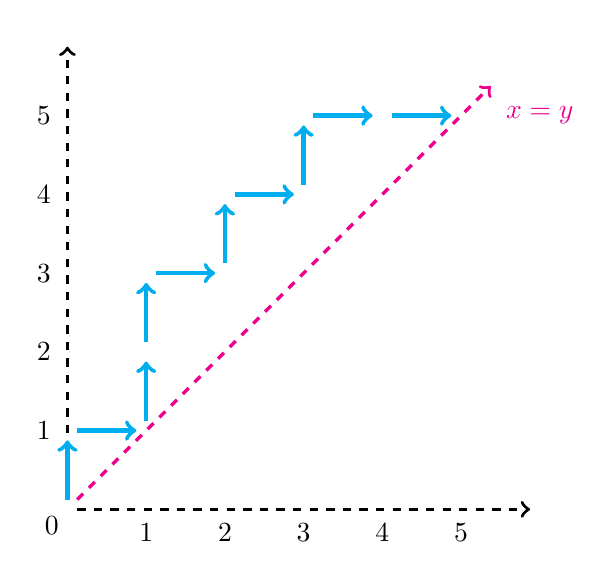
\begin{tikzpicture}[scale=1]
        \node (a) at (0, 0) {};
        \node (b) at (0, 6) {};
        \node (c) at (6, 0) {};
        \node (d) at (5.5, 5.5) {};
        \node (e) at (6, 5) [color = magenta]
            {$x = y$}; 
        \draw [dashed, very thick, ->] (a) to (b);
        \draw [dashed, very thick, ->] (a) to (c);
        \draw [dashed, very thick, ->]
            [color = magenta] (a) to (d);

        \node (1)  at (0,0)   {};
        \node (2)  at (0,1)   {};
        \node (3)  at (1,1)   {};
        \node (4)  at (1,2)   {};
        \node (5)  at (1,3)   {};
        \node (6)  at (2,3)   {};
        \node (7)  at (2,4)   {};
        \node (8)  at (3,4)   {};
        \node (9)  at (3,5)   {};
        \node (10) at (4,5)   {};
        \node (11) at (5,5)   {};
        \draw [->, ultra thick, color = cyan]
            (1)  to (2);
        \draw [->, ultra thick, color = cyan] 
            (2)  to (3);
        \draw [->, ultra thick, color = cyan]
            (3)  to (4);
        \draw [->, ultra thick, color = cyan]
            (4)  to (5);
        \draw [->, ultra thick, color = cyan]
            (5)  to (6);
        \draw [->, ultra thick, color = cyan]
            (6)  to (7);
        \draw [->, ultra thick, color = cyan]
            (7)  to (8);
        \draw [->, ultra thick, color = cyan]
            (8)  to (9);
        \draw [->, ultra thick, color = cyan]
            (9)  to (10);
        \draw [->, ultra thick, color = cyan]
            (10) to (11);

        \node at (-0.2, -0.2) {$0$};
        \node at (-0.3, 1)    {$1$};
        \node at (1, -0.3)    {$1$};
        \node at (-0.3, 2)    {$2$};
        \node at (2, -0.3)    {$2$};
        \node at (-0.3, 3)    {$3$};
        \node at (3, -0.3)    {$3$};
        \node at (-0.3, 4)    {$4$};
        \node at (4, -0.3)    {$4$};
        \node at (-0.3, 5)    {$5$};
        \node at (5, -0.3)    {$5$};

    \end{tikzpicture}
\end{center}
\end{example}

\begin{theorem}
    Let $d_n$ be the cardinal of $\mathcal{D}_n$.
    We have $$d_n = \frac{1}{n + 1} \binom {2n}{n}$$
    which is the $n^{th}$ Catalan number.
\end{theorem}

\begin{example}[$n = 3$]
    $d_n = 5$.
    \begin{center}
        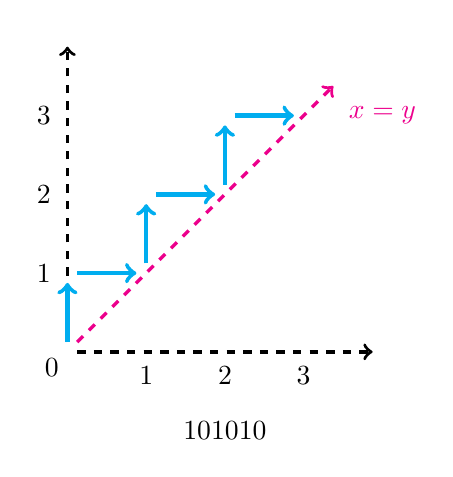
\begin{tikzpicture}[scale = 1]
    \node (a) at (0, 0) {};
    \node (b) at (0, 4) {};
    \node (c) at (4, 0) {};
    \node (d) at (3.5, 3.5) {};
    \node (e) at (4, 3) [color = magenta]
        {$x = y$}; 
    \draw [dashed, very thick, ->] (a) to (b);
    \draw [dashed, very thick, ->] (a) to (c);
    \draw [dashed, very thick, ->]
        [color = magenta] (a) to (d);

    \node (1)  at (0,0)   {};
    \node (2)  at (0,1)   {};
    \node (3)  at (1,1)   {};
    \node (4)  at (1,2)   {};
    \node (5)  at (2,2)   {};
    \node (6)  at (2,3)   {};
    \node (7)  at (3,3)   {};
    \draw [->, ultra thick, color = cyan]
        (1)  to (2);
    \draw [->, ultra thick, color = cyan] 
        (2)  to (3);
    \draw [->, ultra thick, color = cyan]
        (3)  to (4);
    \draw [->, ultra thick, color = cyan]
        (4)  to (5);
    \draw [->, ultra thick, color = cyan]
        (5)  to (6);
    \draw [->, ultra thick, color = cyan]
        (6)  to (7);

    \node at (-0.2, -0.2) {$0$};
    \node at (-0.3, 1)    {$1$};
    \node at (1, -0.3)    {$1$};
    \node at (-0.3, 2)    {$2$};
    \node at (2, -0.3)    {$2$};
    \node at (-0.3, 3)    {$3$};
    \node at (3, -0.3)    {$3$};
    \node at (2, -1)      {$101010$};

\end{tikzpicture}
        \begin{center}
    \begin{tikzpicture}[scale=0.75]
        \node (1)  at (0,16)   {$\{3, 5, 9\}$};
        \node (2)  at (-6,12) {$\{7\}$};
        \node (3)  at (-6,8)  {$\{4, 10\}$};
        \node (5)  at (-5,4)   {$\{1\}$};
        \node (7)  at (0,12)   {$\{2, 8\}$};
        \node (8)  at (-2,8)   {$\{6\}$};
        \node (11) at (6,12)  {$\{11, 12\}$};

        \node (a) at (-1.5,16)    {$1$};
        \node (b) at (-7.5,12)    {$2$};
        \node (c) at (-7.5,8)     {$3$};
        \node (d) at (-7.5,6.15)  {$4$};
        \node (e) at (-6.5,4)     {$5$};
        \node (f) at (-6,2.15)    {$6$};
        \node (g) at (-1.5,12)    {$7$};
        \node (h) at (-3.5,8)     {$8$};
        \node (i) at (-3,6.15)    {$9$};
        \node (j) at (1.75,10.2)  {$10$};
        \node (k) at (7.75,12)    {$11$};
        \node (l) at (4.25,10.2)  {$12$};
        \node (m) at (7.75,10.2)  {$13$};

        \draw[ultra thick][color=brown!70!orange]
            (0,16)  circle (1);
        \draw[ultra thick][color=brown!70!orange]
            (-6,12) circle (1);
        \draw[ultra thick][color=brown!70!orange]
            (-6,8)  circle (1);
        \draw[ultra thick][color=brown!70!orange]
            (-5,4)  circle (1);
        \draw[ultra thick][color=brown!70!orange]
            (0,12)  circle (1);
        \draw[ultra thick][color=brown!70!orange]
            (-2,8)  circle (1);
        \draw[ultra thick][color=brown!70!orange]
            (6,12)  circle (1);

        \draw [->][ultra thick][color=brown!70!orange]
            (-0.5,15.15) to (-6,13.2);
        \draw [->][ultra thick][color=brown!70!orange]
            (0,15) to (0,13.2);
        \draw [->][ultra thick][color=brown!70!orange]
            (0.5,15.15) to (6,13.2);
        \draw [->][ultra thick][color=brown!70!orange]
            (-6,11) to (-6,9.2);
        \draw [->][ultra thick][color=brown!70!orange]
            (-0.25,11) to (-2,9.2);
        \draw [->][ultra thick][color=brown!70!orange]
            (-5.75,7) to (-5,5.2);

        \draw [-*][ultra thick][color=green!60!gray]
            (-6.25,7) to (-6.75,6);
        \draw [-*][ultra thick][color=green!60!gray]
            (-5,3) to (-5, 2);
        \draw [-*][ultra thick][color=green!60!gray]
            (-2,7) to (-2,6);
        \draw [-*][ultra thick][color=green!60!gray]
            (0.25,11) to (0.75,10);
        \draw [-*][ultra thick][color=green!60!gray]
            (5.75,11) to (5.25,10);
        \draw [-*][ultra thick][color=green!60!gray]
            (6.25,11) to (6.75,10);
    \end{tikzpicture}
\end{center}
        ~
\begin{center}
    \begin{tikzpicture}[scale=0.75]
        \node (1)  at (0,16)   {$\{5\}$};
        \node (2)  at (0,12)   {$\{2\}$};
        \node (3)  at (0,8)   {$\{1,3,4,7\}$};
        \node (6)  at (1,4)    {$\{8\}$};
        \node (7)  at (1,0)   {$\{6\}$};

        \node (a) at (-1.5,16)    {$1$};
        \node (b) at (-1.5,12)    {$2$};
        \node (c) at (-1.5,8)     {$3$};
        \node (d) at (-1.5,5.5)   {$4$};
        \node (e) at (-0.5,5.5)   {$5$};
        \node (f) at (-0.5,4)     {$6$};
        \node (g) at (-0.5,0)     {$7$};
        \node (h) at (0,-1.5)     {$8$};
        \node (i) at (1.5,5.5)    {$9$};

        \draw[ultra thick][color=brown!70!orange]
            (0,16)  circle (1);
        \draw[ultra thick][color=brown!70!orange]
            (0,12) circle (1);
        \draw[ultra thick][color=brown!70!orange]
            (0,8)  circle (1);
        \draw[ultra thick][color=brown!70!orange]
            (1,4)  circle (1);
        \draw[ultra thick][color=brown!70!orange]
            (1,0)  circle (1);

        \draw [->][ultra thick][color=brown!70!orange]
            (0,15) to (0,13.2);
        \draw [->][ultra thick][color=brown!70!orange]
            (0,11) to (0,9.2);
        \draw [->][ultra thick][color=brown!70!orange]
            (0.2,7) to (1,5.2);
        \draw [->][ultra thick][color=brown!70!orange]
            (1,3) to (1,1.2);

        \draw [-*][ultra thick][color=green!60!gray]
            (-0.5,7.15) to (-1.5,6);
        \draw [-*][ultra thick][color=green!60!gray]
            (-0.25,7.05) to (-0.5, 6);
        \draw [-*][ultra thick][color=green!60!gray]
            (0.5,7.15) to (1.5,6);
        \draw [-*][ultra thick][color=green!60!gray]
            (1,-1) to (1,-2);
    \end{tikzpicture}
\end{center}  
        
        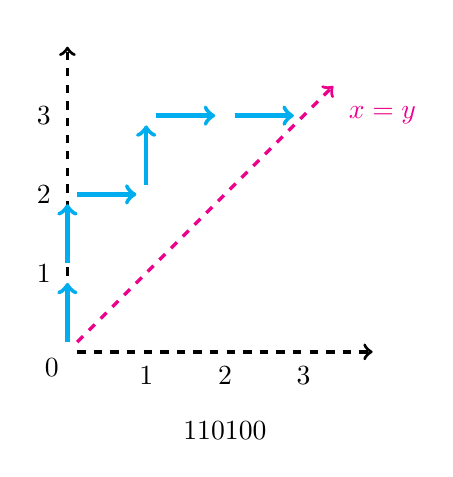
\begin{tikzpicture}[scale = 1]
            \node (a) at (0, 0) {};
            \node (b) at (0, 4) {};
            \node (c) at (4, 0) {};
            \node (d) at (3.5, 3.5) {};
            \node (e) at (4, 3) [color = magenta]
                {$x = y$}; 
            \draw [dashed, very thick, ->] (a) to (b);
            \draw [dashed, very thick, ->] (a) to (c);
            \draw [dashed, very thick, ->]
                [color = magenta] (a) to (d);

            \node (1)  at (0,0)   {};
            \node (2)  at (0,1)   {};
            \node (3)  at (0,2)   {};
            \node (4)  at (1,2)   {};
            \node (5)  at (1,3)   {};
            \node (6)  at (2,3)   {};
            \node (7)  at (3,3)   {};
            \draw [->, ultra thick, color = cyan]
                (1)  to (2);
            \draw [->, ultra thick, color = cyan] 
                (2)  to (3);
            \draw [->, ultra thick, color = cyan]
                (3)  to (4);
            \draw [->, ultra thick, color = cyan]
                (4)  to (5);
            \draw [->, ultra thick, color = cyan]
                (5)  to (6);
            \draw [->, ultra thick, color = cyan]
                (6)  to (7);

            \node at (-0.2, -0.2) {$0$};
            \node at (-0.3, 1)    {$1$};
            \node at (1, -0.3)    {$1$};
            \node at (-0.3, 2)    {$2$};
            \node at (2, -0.3)    {$2$};
            \node at (-0.3, 3)    {$3$};
            \node at (3, -0.3)    {$3$};
            \node at (2, -1)      {$110100$};
        \end{tikzpicture}
        \begin{center}
    \begin{tikzpicture}[scale=0.75]
        \node (1)  at (0,17)   {$\{4,9\}$};
        \node (2)  at (0,13)   {$\{2,3\}$};
        \node (4)  at (3,9)   {$\{1,5,8\}$};
        \node (5)  at (0,5)    {$\{6\}$};
        \node (7)  at (6,5)    {$\{7\}$};

        \node (a) at (-1.5,17)    {$1$};
        \node (b) at (-1.5,13)    {$2$};
        \node (c) at (-2,11)      {$3$};
        \node (d) at (1.5,9)      {$4$};
        \node (e) at (1.5,5)      {$5$};
        \node (f) at (-1,3)       {$6$};
        \node (g) at (4.5,5)      {$7$};
        \node (h) at (5,3)        {$8$};

        \node[right] (ac) at (1.5,17) {$2$ groupes d'enfants : $\emptyset$
         et $[2]$};
        \node[right] (bc) at (1.5,13) {$2$ groupes d'enfants : $[3]$
         et $[4]$};
        \node[right] (dc) at (4.5,9) {$3$ groupes d'enfants : $\emptyset$,
         $[5]$ et $[7]$};
        \node[left] (fc) at (-1.5,5) {$1$ groupe d'enfants : $[6]$};
        \node[right] (gc) at (7.5,5) {$1$ groupe d'enfants : $[8]$};

        \draw[ultra thick][color=brown!70!orange]
            (0,17)  circle (1);
        \draw[ultra thick][color=brown!70!orange]
            (0,13) circle (1);
        \draw[ultra thick][color=brown!70!orange]
            (3,9)  circle (1);
        \draw[ultra thick][color=brown!70!orange]
            (0,5)  circle (1);
        \draw[ultra thick][color=brown!70!orange]
            (6,5)  circle (1);

        \draw [->][ultra thick][color=brown!70!orange]
            (0,16) to (0,14.2);
        \draw [->][ultra thick][color=brown!70!orange]
            (0.6,12.25) to (2.7,10.2);
        \draw [->][ultra thick][color=brown!70!orange]
            (2.4,8.25) to (0.3,6.2);
        \draw [->][ultra thick][color=brown!70!orange]
            (3.6,8.25) to (5.7,6.2);

        \draw [-*][ultra thick][color=green!60!gray]
            (-0.6,12.2) to (-1.6,11);
        \draw [-*][ultra thick][color=green!60!gray]
            (0,4) to (0,3);
        \draw [-*][ultra thick][color=green!60!gray]
            (6,4) to (6,3);
    \end{tikzpicture}
\end{center}
    \end{center}
\end{example}

\begin{prop}
    This means we can create a \emph{bijection} between
    $\mathcal{PF'}_n$ and $\mathcal{D}_n$.
\end{prop}

\begin{proof}
    ~\
\begin{itemize}
    \item $\mathcal{PF'}_n \to \mathcal{D}_n$ :
    Let $f = (a_1, \ldots, a_n) \in \mathcal{PF'}_n$
    be our primitive parking function.
    For $i \in \{1, \ldots, n\}$, we define $l_i$ the
    number of occurences of $i$ in $f$.\\
    The corresponding Dyck word will be
    $\underbrace{1 \cdots 1}_{l_1}0
     \underbrace{1 \cdots 1}_{l_2}0 \cdots
     \underbrace{1 \cdots 1}_{l_n}0$.
    
    \item $\mathcal{D}_n \to \mathcal{PF'}_n$ :
    Let $w$ be our Dyck word, and consider its path
    representation. We define $s_i$ to be the distance
    between the segment from $(0, i - 1)$ to $(0, i)$
    and the $i^{th}$ North step. Then, let $a_i = s_i + 1$.\\
    The corresponding primitive parking function is 
    $(a_1, \ldots, a_n)$.
\end{itemize}
\end{proof}

\begin{example}[$n = 6, \mathcal{PF'}_n \to \mathcal{D}_n$]
    ~\
    \begin{itemize}
        \item $f = (1, 1, 2, 4, 5, 5)$
            \subitem $l_1 = 2$
            \hspace{2cm} $l_2 = 1$
            \hspace{2cm} $l_3 = 0$
            \subitem $l_4 = 1$
            \hspace{2cm} $l_5 = 2$
            \hspace{2cm} $l_6 = 0$
        \item $w = (110100101100)$
    \end{itemize}
    \begin{center}
    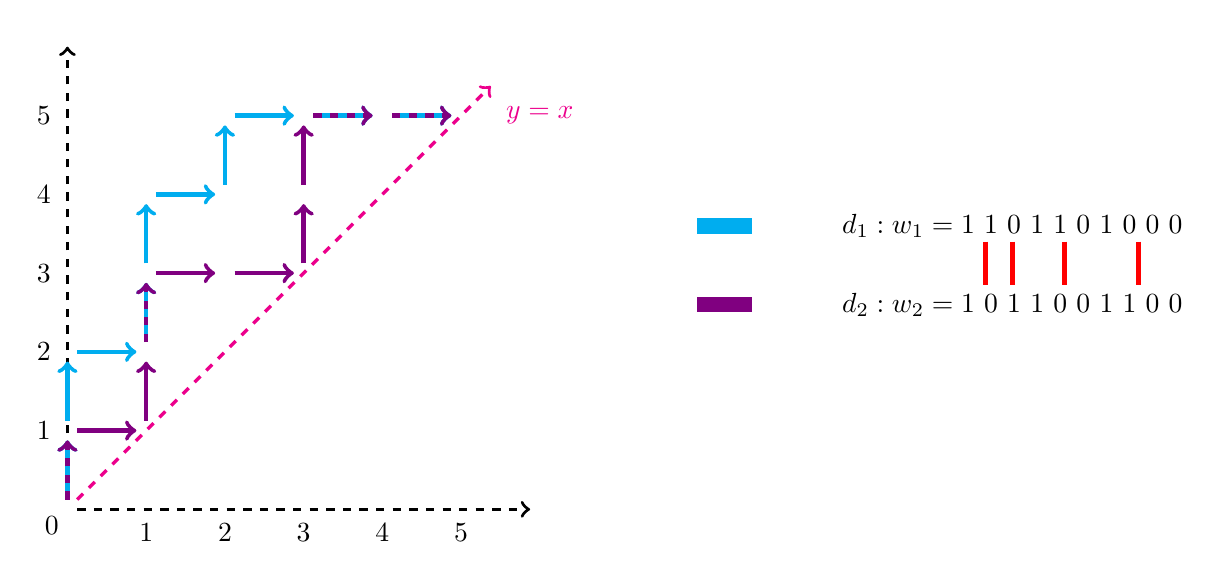
\begin{tikzpicture}[scale=1]
        \node (a) at (0, 0) {};
        \node (b) at (0, 6) {};
        \node (c) at (6, 0) {};
        \node (d) at (5.5, 5.5) {};
        \node (e) at (6, 5) [color = magenta] {$y = x$}; 
        \draw [dashed, very thick, ->] (a) to (b);
        \draw [dashed, very thick, ->] (a) to (c);
        \draw [dashed, very thick, ->]
            [color = magenta] (a) to (d);

        \node (1)  at (0,0)   {};
        \node (2)  at (0,1)   {};
        \node (3)  at (0,2)   {};
        \node (3b) at (1, 1)  {};
        \node (4)  at (1,2)   {};
        \node (5)  at (1,3)   {};
        \node (6)  at (1,4)   {};
        \node (6b) at (2,3)   {};
        \node (7)  at (2,4)   {};
        \node (7b) at (3,3)   {};
        \node (8)  at (2,5)   {};
        \node (8b) at (3, 4)  {};
        \node (9)  at (3,5)   {};
        \node (10) at (4,5)   {};
        \node (11) at (5,5)   {};

        \draw [->, ultra thick, color = cyan]
            (1)  to (2);
        \draw [->, ultra thick, color = cyan] 
            (2)  to (3);
        \draw [->, ultra thick, color = cyan]
            (3)  to (4);
        \draw [->, ultra thick, color = cyan]
            (4)  to (5);
        \draw [->, ultra thick, color = cyan]
            (5)  to (6);
        \draw [->, ultra thick, color = cyan]
            (6)  to (7);
        \draw [->, ultra thick, color = cyan]
            (7)  to (8);
        \draw [->, ultra thick, color = cyan]
            (8)  to (9);
        \draw [->, ultra thick, color = cyan]
            (9)  to (10);
        \draw [->, ultra thick, color = cyan]
            (10) to (11);

        \draw [->, dashed, ultra thick, color = violet]
            (1)  to (2);
        \draw [->, ultra thick, color = violet] 
            (2)  to (3b);
        \draw [->, ultra thick, color = violet]
            (3b)  to (4);
        \draw [->, dashed, ultra thick, color = violet]
            (4)  to (5);
        \draw [->, ultra thick, color = violet]
            (5)  to (6b);
        \draw [->, ultra thick, color = violet]
            (6b)  to (7b);
        \draw [->, ultra thick, color = violet]
            (7b)  to (8b);
        \draw [->, ultra thick, color = violet]
            (8b)  to (9);
        \draw [->, dashed, ultra thick, color = violet]
            (9)  to (10);
        \draw [->, dashed, ultra thick, color = violet]
            (10) to (11);

        \node at (-0.2, -0.2) {$0$};
        \node at (-0.3, 1)    {$1$};
        \node at (1, -0.3)    {$1$};
        \node at (-0.3, 2)    {$2$};
        \node at (2, -0.3)    {$2$};
        \node at (-0.3, 3)    {$3$};
        \node at (3, -0.3)    {$3$};
        \node at (-0.3, 4)    {$4$};
        \node at (4, -0.3)    {$4$};
        \node at (-0.3, 5)    {$5$};
        \node at (5, -0.3)    {$5$};

    \fill[color = cyan] (8,3.5) rectangle (8.7,3.7);
    \node at (12,3.6) {$d_1 : w_1 = 1\ 1\ 0\ 1\ 1\ 0\ 1\ 0\ 0\ 0$};
    \fill[color = violet] (8,2.5) rectangle (8.7,2.7);
    \node at (12,2.6) {$d_2 : w_2 = 1\ 0\ 1\ 1\ 0\ 0\ 1\ 1\ 0\ 0$};

    \draw [-, ultra thick, color = red] (11.66,3.4) to (11.66,2.85);
    \draw [-, ultra thick, color = red] (12,3.4) to (12,2.85);
    \draw [-, ultra thick, color = red] (12.66,3.4) to (12.66,2.85);
    \draw [-, ultra thick, color = red] (13.6,3.4) to (13.6,2.85);

    \end{tikzpicture}
\end{center}
\end{example}

\begin{example}[$n = 6, \mathcal{D}_n \to \mathcal{PF'}_n$]
    ~\
    \begin{itemize}
        \item $w = 101011010010$
    \end{itemize}
    
    \begin{center}
        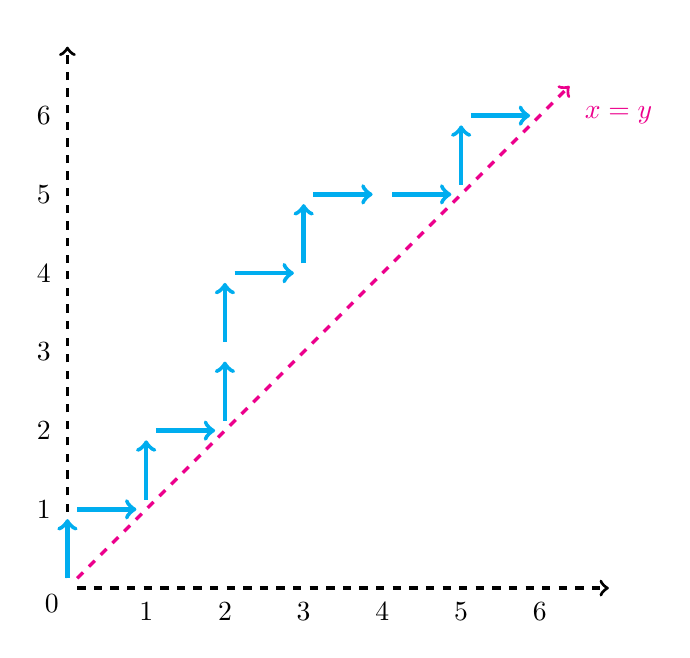
\begin{tikzpicture}[scale=1]
            \node (a) at (0, 0) {};
            \node (b) at (0, 7) {};
            \node (c) at (7, 0) {};
            \node (d) at (6.5, 6.5) {};
            \node (e) at (7, 6) [color = magenta]
                {$x = y$}; 
            \draw [dashed, very thick, ->] (a) to (b);
            \draw [dashed, very thick, ->] (a) to (c);
            \draw [dashed, very thick, ->]
                [color = magenta] (a) to (d);

            \node (1)  at (0,0)   {};
            \node (2)  at (0,1)   {};
            \node (3)  at (1,1)   {};
            \node (4)  at (1,2)   {};
            \node (5)  at (2,2)   {};
            \node (6)  at (2,3)   {};
            \node (7)  at (2,4)   {};
            \node (8)  at (3,4)   {};
            \node (9)  at (3,5)   {};
            \node (10) at (4,5)   {};
            \node (11) at (5,5)   {};
            \node (12) at (5,6)   {};
            \node (13) at (6,6)   {};
            \draw [->, ultra thick, color = cyan]
                (1)  to (2);
            \draw [->, ultra thick, color = cyan] 
                (2)  to (3);
            \draw [->, ultra thick, color = cyan]
                (3)  to (4);
            \draw [->, ultra thick, color = cyan]
                (4)  to (5);
            \draw [->, ultra thick, color = cyan]
                (5)  to (6);
            \draw [->, ultra thick, color = cyan]
                (6)  to (7);
            \draw [->, ultra thick, color = cyan]
                (7)  to (8);
            \draw [->, ultra thick, color = cyan]
                (8)  to (9);
            \draw [->, ultra thick, color = cyan]
                (9)  to (10);
            \draw [->, ultra thick, color = cyan]
                (10) to (11);
            \draw [->, ultra thick, color = cyan]
                (11) to (12);
            \draw [->, ultra thick, color = cyan]
                (12) to (13);

            \node at (-0.2, -0.2) {$0$};
            \node at (-0.3, 1)    {$1$};
            \node at (1, -0.3)    {$1$};
            \node at (-0.3, 2)    {$2$};
            \node at (2, -0.3)    {$2$};
            \node at (-0.3, 3)    {$3$};
            \node at (3, -0.3)    {$3$};
            \node at (-0.3, 4)    {$4$};
            \node at (4, -0.3)    {$4$};
            \node at (-0.3, 5)    {$5$};
            \node at (5, -0.3)    {$5$};
            \node at (-0.3, 6)    {$6$};
            \node at (6, -0.3)    {$6$};

        \end{tikzpicture}
    \end{center}
    \begin{itemize}
        \item Distances : 
            \subitem $s_1 = 0$
                \hspace{2cm} $a_1 = 1$
            \subitem $s_2 = 1$
                \hspace{2cm} $a_2 = 2$
            \subitem $s_3 = 2$
                \hspace{2cm} $a_3 = 3$
            \subitem $s_4 = 2$
                \hspace{2cm} $a_4 = 3$
            \subitem $s_5 = 3$
                \hspace{2cm} $a_5 = 4$
            \subitem $s_6 = 5$
                \hspace{2cm} $a_6 = 6$
        \item $f = (1, 2, 3, 3, 4, 6)$
    \end{itemize}
    
\end{example}

\subsection{Labeled Dyck Paths}

\begin{definition}[Labeled Dyck Path]
    A \emph{labeled Dyck word} is a word $w \in 
    \{0, \ldots, n\}^*$ such that :
    \begin{itemize}
        \item for each suffix $w'$ of $w$,
            $|w'|_{\neq 0} \geqslant |w'|_0$.
        \item $|w|_0 = |w|_{\neq 0}$.
        \item for each $i \in \{1, \ldots, n\}$, $w$ has 
            exactly one occurence of $i$.
        \item if $w_i \neq 0$ and $w_{i+1} \neq 0$,
            then $w_i < w_{i+1}$. That is, consecutive
            North steps have increasing labels.
    \end{itemize}
    A labeled Dyck word of length $2n$ can be represented
    as a path from $(0,0)$ to $(n,n)$, where each North
    step is associated to a label :
    \begin{itemize}
        \item Each $i \neq 0$ corresponds to a
            \emph{North step} $\uparrow$ labeled $i$.
        \item Each $0$ corresponds to an
            \emph{East step} $\rightarrow$.
    \end{itemize}
    Those paths are called \emph{labeled Dyck paths}.\\
    We denote by $\mathcal{LD}_n$ the set of labeled
    Dyck words of length $2n$.
\end{definition}

\begin{example}[$n = 5$]
    \begin{align*}
        &w_1 = 4051002030 \text{ is \emph{not} a labeled
            Dyck word, because }5 > 1.\\
        &w_2 = 4015002030 \text{ \emph{is} a labeled
            Dyck word :}\\
    \end{align*}
    \begin{center}
    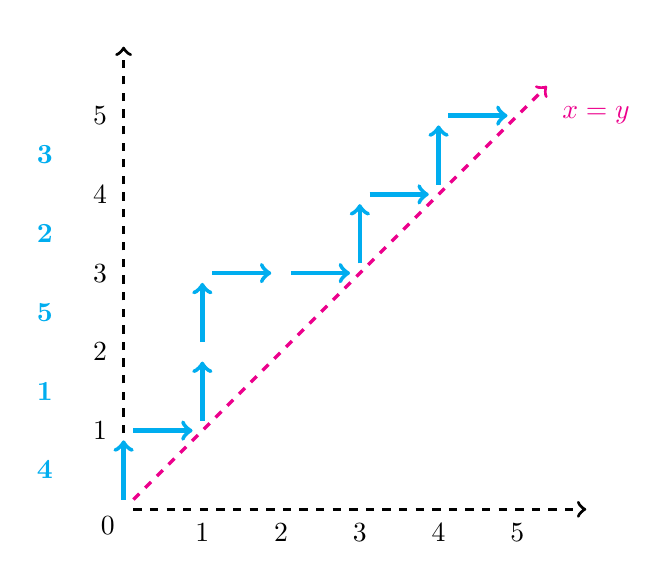
\begin{tikzpicture}[scale=1]
        \node (a) at (0, 0) {};
        \node (b) at (0, 6) {};
        \node (c) at (6, 0) {};
        \node (d) at (5.5, 5.5) {};
        \node (e) at (6, 5) [color = magenta]
            {$x = y$}; 
        \draw [dashed, very thick, ->] (a) to (b);
        \draw [dashed, very thick, ->] (a) to (c);
        \draw [dashed, very thick, ->]
            [color = magenta] (a) to (d);

        \node (1)  at (0,0)   {};
        \node (2)  at (0,1)   {};
        \node (3)  at (1,1)   {};
        \node (4)  at (1,2)   {};
        \node (5)  at (1,3)   {};
        \node (6)  at (2,3)   {};
        \node (7)  at (3,3)   {};
        \node (8)  at (3,4)   {};
        \node (9)  at (4,4)   {};
        \node (10) at (4,5)   {};
        \node (11) at (5,5)   {};
        \draw [->, ultra thick, color = cyan]
            (1)  to (2);
        \draw [->, ultra thick, color = cyan] 
            (2)  to (3);
        \draw [->, ultra thick, color = cyan]
            (3)  to (4);
        \draw [->, ultra thick, color = cyan]
            (4)  to (5);
        \draw [->, ultra thick, color = cyan]
            (5)  to (6);
        \draw [->, ultra thick, color = cyan]
            (6)  to (7);
        \draw [->, ultra thick, color = cyan]
            (7)  to (8);
        \draw [->, ultra thick, color = cyan]
            (8)  to (9);
        \draw [->, ultra thick, color = cyan]
            (9)  to (10);
        \draw [->, ultra thick, color = cyan]
            (10) to (11);

        \node at (-0.2, -0.2) {$0$};
        \node at (-0.3, 1)    {$1$};
        \node at (1, -0.3)    {$1$};
        \node at (-0.3, 2)    {$2$};
        \node at (2, -0.3)    {$2$};
        \node at (-0.3, 3)    {$3$};
        \node at (3, -0.3)    {$3$};
        \node at (-0.3, 4)    {$4$};
        \node at (4, -0.3)    {$4$};
        \node at (-0.3, 5)    {$5$};
        \node at (5, -0.3)    {$5$};

        \node [color = cyan] at (-1, 0.5) {\textbf{4}};
        \node [color = cyan] at (-1, 1.5) {\textbf{1}};
        \node [color = cyan] at (-1, 2.5) {\textbf{5}};
        \node [color = cyan] at (-1, 3.5) {\textbf{2}};
        \node [color = cyan] at (-1, 4.5) {\textbf{3}};

    \end{tikzpicture}
\end{center}
\end{example}

\begin{theorem}
    Let $ld_n$ be the cardinal of $\mathcal{LD}_n$.
    We have $$ld_n = (n + 1)^{n - 1}$$.
\end{theorem}

\begin{example}[$n = 3$]
    $ld_n = 4^2 = 16$
    \begin{itemize}
        \item Word of shape $XXX000$ :
            \subitem $123000$
        \item Words of shape $XX0X00$ :
            \subitem $120300$
            \hspace{2cm} $130200$
            \hspace{2cm} $230100$
        \item Words of shape $XX00X0$ :
            \subitem $120030$
            \hspace{2cm} $130020$
            \hspace{2cm} $230010$
        \item Words of shape $X0XX00$ :
            \subitem $102300$
            \hspace{2cm} $201300$
            \hspace{2cm} $301200$
        \item Words of shape $X0X0X0$ :
            \subitem $102030$
            \hspace{2cm} $103020$
            \hspace{2cm} $201030$
            \subitem $203010$
            \hspace{2cm} $301020$
            \hspace{2cm} $302010$
    \end{itemize}
    
\end{example}

\begin{prop}
    This means we can create a \emph{bijection} between
    $\mathcal{PF}_n$ and $\mathcal{LD}_n$.
\end{prop}

\begin{proof}
    ~\
    \begin{itemize}
        \item $\mathcal{PF}_n \to \mathcal{LD}_n$ :
        Let $f = (a_1, \ldots, a_n) \in \mathcal{PF}_n$
        be our parking function. For $i \in \{1, \ldots,
        n\}$, we define $im_i$ : $\{j\ |\ a_j = i\}$. \\
        We then define $im_{i,1}, \ldots, im_{i,k_i}$ to be
        the elements of $im_i$ in increasing order.\\
        The corresponding labeled Dyck word will be \\
        $\underbrace{im_{1,1} \cdots im_{1,k_1}}_{im_1}0
         \underbrace{im_{2,1} \cdots im_{2,k_2}}_{im_2}0
         \cdots
         \underbrace{im_{n,1} \cdots im_{n,k_n}}_{im_n}0$.

        \item $\mathcal{LD}_n \to \mathcal{PF}_n$ :
        Let w be our labeled Dyck word, and consider its
        path representation. We define $s_i$ to be the
        distance between the segment from $(0, i-1)$ to
        $(0,i)$ and the $i^{th}$ North step.\\
        Then, let $label(i)$ be the label of the $i^{th}$
        North step, and $dist_i = \{label(j) | s_j = i\}$
        be the set of the labels of all North steps at
        distance $i$.\\
        Then, if $j \in dist_i$, let $a_j = i + 1$.\\
        The corresponding parking function is
        $(a_1, \ldots, a_n)$.
    \end{itemize}
\end{proof}

\begin{example}[$n = 6, \mathcal{PF}_n \to \mathcal{LD}_n$]
    ~\
    \begin{itemize}
        \item $f = (5, 2, 1, 4, 5, 1)$
            \subitem $im_1 = \{3, 6\}$
            \hspace{16mm} $im_2 = \{2\}$
            \hspace{24mm} $im_3 = \emptyset$
            \subitem $im_4 = \{4\}$
            \hspace{2cm} $im_5 = \{1, 5\}$
            \hspace{2cm} $im_6 = \emptyset$
        \item $w = 360200401500$
    \end{itemize}
    \begin{center}
    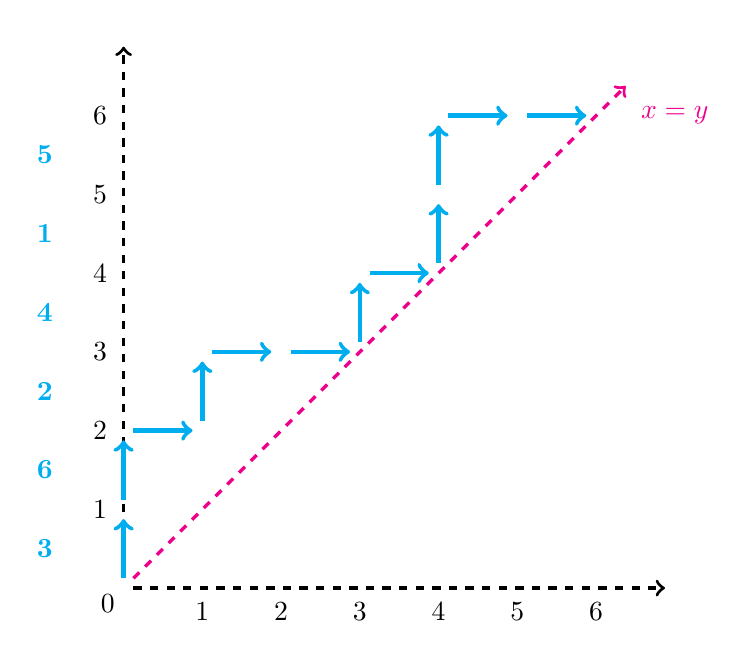
\begin{tikzpicture}[scale=1]
        \node (a) at (0, 0) {};
        \node (b) at (0, 7) {};
        \node (c) at (7, 0) {};
        \node (d) at (6.5, 6.5) {};
        \node (e) at (7, 6) [color = magenta]
            {$x = y$}; 
        \draw [dashed, very thick, ->] (a) to (b);
        \draw [dashed, very thick, ->] (a) to (c);
        \draw [dashed, very thick, ->]
            [color = magenta] (a) to (d);

        \node (1)  at (0,0)   {};
        \node (2)  at (0,1)   {};
        \node (3)  at (0,2)   {};
        \node (4)  at (1,2)   {};
        \node (5)  at (1,3)   {};
        \node (6)  at (2,3)   {};
        \node (7)  at (3,3)   {};
        \node (8)  at (3,4)   {};
        \node (9)  at (4,4)   {};
        \node (10) at (4,5)   {};
        \node (11) at (4,6)   {};
        \node (12) at (5,6)   {};
        \node (13) at (6,6)   {};
        \draw [->, ultra thick, color = cyan]
            (1)  to (2);
        \draw [->, ultra thick, color = cyan] 
            (2)  to (3);
        \draw [->, ultra thick, color = cyan]
            (3)  to (4);
        \draw [->, ultra thick, color = cyan]
            (4)  to (5);
        \draw [->, ultra thick, color = cyan]
            (5)  to (6);
        \draw [->, ultra thick, color = cyan]
            (6)  to (7);
        \draw [->, ultra thick, color = cyan]
            (7)  to (8);
        \draw [->, ultra thick, color = cyan]
            (8)  to (9);
        \draw [->, ultra thick, color = cyan]
            (9)  to (10);
        \draw [->, ultra thick, color = cyan]
            (10) to (11);
        \draw [->, ultra thick, color = cyan]
            (11) to (12);
        \draw [->, ultra thick, color = cyan]
            (12) to (13);

        \node at (-0.2, -0.2) {$0$};
        \node at (-0.3, 1)    {$1$};
        \node at (1, -0.3)    {$1$};
        \node at (-0.3, 2)    {$2$};
        \node at (2, -0.3)    {$2$};
        \node at (-0.3, 3)    {$3$};
        \node at (3, -0.3)    {$3$};
        \node at (-0.3, 4)    {$4$};
        \node at (4, -0.3)    {$4$};
        \node at (-0.3, 5)    {$5$};
        \node at (5, -0.3)    {$5$};
        \node at (-0.3, 6)    {$6$};
        \node at (6, -0.3)    {$6$};

        \node [color = cyan] at (-1, 0.5) {\textbf{3}};
        \node [color = cyan] at (-1, 1.5) {\textbf{6}};
        \node [color = cyan] at (-1, 2.5) {\textbf{2}};
        \node [color = cyan] at (-1, 3.5) {\textbf{4}};
        \node [color = cyan] at (-1, 4.5) {\textbf{1}};
        \node [color = cyan] at (-1, 5.5) {\textbf{5}};
    \end{tikzpicture}
\end{center}
\end{example}

\begin{example}[$n = 6, \mathcal{LD}_n \to \mathcal{PF}_n$]
    ~\
    \begin{itemize}
        \item $w = 402560010030$
    \end{itemize}
    \begin{center}
    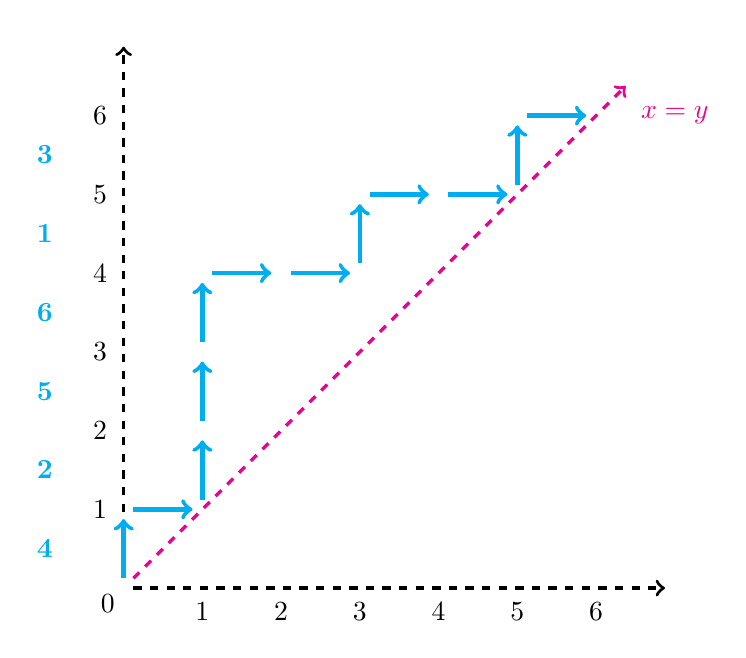
\begin{tikzpicture}[scale=1]
        \node (a) at (0, 0) {};
        \node (b) at (0, 7) {};
        \node (c) at (7, 0) {};
        \node (d) at (6.5, 6.5) {};
        \node (e) at (7, 6) [color = magenta]
            {$x = y$}; 
        \draw [dashed, very thick, ->] (a) to (b);
        \draw [dashed, very thick, ->] (a) to (c);
        \draw [dashed, very thick, ->]
            [color = magenta] (a) to (d);

        \node (1)  at (0,0)   {};
        \node (2)  at (0,1)   {};
        \node (3)  at (1,1)   {};
        \node (4)  at (1,2)   {};
        \node (5)  at (1,3)   {};
        \node (6)  at (1,4)   {};
        \node (7)  at (2,4)   {};
        \node (8)  at (3,4)   {};
        \node (9)  at (3,5)   {};
        \node (10) at (4,5)   {};
        \node (11) at (5,5)   {};
        \node (12) at (5,6)   {};
        \node (13) at (6,6)   {};
        \draw [->, ultra thick, color = cyan]
            (1)  to (2);
        \draw [->, ultra thick, color = cyan] 
            (2)  to (3);
        \draw [->, ultra thick, color = cyan]
            (3)  to (4);
        \draw [->, ultra thick, color = cyan]
            (4)  to (5);
        \draw [->, ultra thick, color = cyan]
            (5)  to (6);
        \draw [->, ultra thick, color = cyan]
            (6)  to (7);
        \draw [->, ultra thick, color = cyan]
            (7)  to (8);
        \draw [->, ultra thick, color = cyan]
            (8)  to (9);
        \draw [->, ultra thick, color = cyan]
            (9)  to (10);
        \draw [->, ultra thick, color = cyan]
            (10) to (11);
        \draw [->, ultra thick, color = cyan]
            (11) to (12);
        \draw [->, ultra thick, color = cyan]
            (12) to (13);

        \node at (-0.2, -0.2) {$0$};
        \node at (-0.3, 1)    {$1$};
        \node at (1, -0.3)    {$1$};
        \node at (-0.3, 2)    {$2$};
        \node at (2, -0.3)    {$2$};
        \node at (-0.3, 3)    {$3$};
        \node at (3, -0.3)    {$3$};
        \node at (-0.3, 4)    {$4$};
        \node at (4, -0.3)    {$4$};
        \node at (-0.3, 5)    {$5$};
        \node at (5, -0.3)    {$5$};
        \node at (-0.3, 6)    {$6$};
        \node at (6, -0.3)    {$6$};

        \node [color = cyan] at (-1, 0.5) {\textbf{4}};
        \node [color = cyan] at (-1, 1.5) {\textbf{2}};
        \node [color = cyan] at (-1, 2.5) {\textbf{5}};
        \node [color = cyan] at (-1, 3.5) {\textbf{6}};
        \node [color = cyan] at (-1, 4.5) {\textbf{1}};
        \node [color = cyan] at (-1, 5.5) {\textbf{3}};
    \end{tikzpicture}
\end{center}
    \begin{itemize}
        \item Distances :
            \subitem $s_1 = 0$
            \hspace{2cm} $s_2 = 1$
            \hspace{2cm} $s_3 = 1$
            \subitem $s_4 = 1$
            \hspace{2cm} $s_5 = 3$
            \hspace{2cm} $s_6 = 5$
        \item Labels :
            \subitem $dist_0 = \{4\}$
            \hspace{2cm} $dist_1 = \{2, 5, 6\}$
            \hspace{2cm} $dist_2 = \emptyset$
            \subitem $dist_3 = \{1\}$
            \hspace{2cm} $dist_4 = \emptyset$
            \hspace{32mm} $dist_5 = \{3\}$
        \item $f = (4, 2, 6, 1, 2, 2)$
    \end{itemize}
\end{example}

\begin{rem}
    The primitive parking functions are exactly the
    parking functions corresponding to labeled Dyck paths
    where the $i^{th}$ North step is labeled $i$.
\end{rem}

\subsection{Dyck - Parking Posets}

\subsubsection{Primitive Dyck - Parking Posets}

\begin{definition}[$\gtrdot_d$]
    For $w$ and $w'$ two Dyck words, we say that $w$
    covers $w'$, written $w \gtrdot_d w'$, if
    $\exists w_1, w_2$ such that :
    \begin{itemize}
        \item $w = w_101w_2$
        \item $w' = w_110w_2$
    \end{itemize}  
\end{definition}

\begin{example}[$n = 7$]
    $10110011001100 \gtrdot_d 10110101001100$
    \begin{itemize}
        \item $w_1 = 10110$
        \item $w_2 = 1001100$
    \end{itemize}
    \begin{center}
    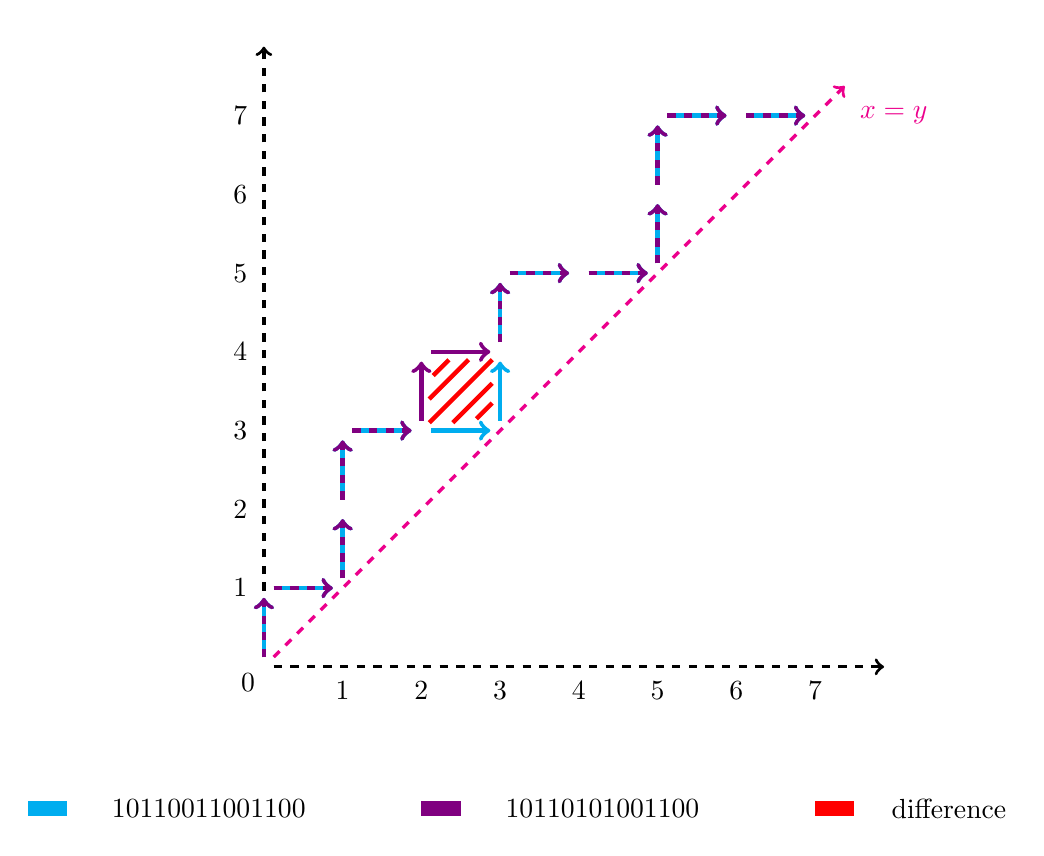
\begin{tikzpicture}[scale=1]
        \node (a) at (0, 0) {};
        \node (b) at (0, 8) {};
        \node (c) at (8, 0) {};
        \node (d) at (7.5, 7.5) {};
        \node (e) at (8, 7) [color = magenta]
            {$x = y$}; 
        \draw [dashed, very thick, ->] (a) to (b);
        \draw [dashed, very thick, ->] (a) to (c);
        \draw [dashed, very thick, ->]
            [color = magenta] (a) to (d);

        \node (1)  at (0,0)   {};
        \node (2)  at (0,1)   {};
        \node (3)  at (1,1)   {};
        \node (4)  at (1,2)   {};
        \node (5)  at (1,3)   {};
        \node (6)  at (2,3)   {};
        \node (7)  at (3,3)   {};
        \node (7b) at (2,4)   {};
        \node (8)  at (3,4)   {};
        \node (9)  at (3,5)   {};
        \node (10) at (4,5)   {};
        \node (11) at (5,5)   {};
        \node (12) at (5,6)   {};
        \node (13) at (5,7)   {};
        \node (14) at (6,7)   {};
        \node (15) at (7,7)   {};

        \draw [->, ultra thick, color = cyan]
            (1)  to (2);
        \draw [->, ultra thick, color = cyan] 
            (2)  to (3);
        \draw [->, ultra thick, color = cyan]
            (3)  to (4);
        \draw [->, ultra thick, color = cyan]
            (4)  to (5);
        \draw [->, ultra thick, color = cyan]
            (5)  to (6);
        \draw [->, ultra thick, color = cyan]
            (6)  to (7);
        \draw [->, ultra thick, color = cyan]
            (7)  to (8);
        \draw [->, ultra thick, color = cyan]
            (8)  to (9);
        \draw [->, ultra thick, color = cyan]
            (9)  to (10);
        \draw [->, ultra thick, color = cyan]
            (10) to (11);
        \draw [->, ultra thick, color = cyan]
            (11) to (12);
        \draw [->, ultra thick, color = cyan]
            (12) to (13);
        \draw [->, ultra thick, color = cyan]
            (13) to (14);
        \draw [->, ultra thick, color = cyan]
            (14) to (15);

        \draw [->, dashed, ultra thick, color = violet]
            (1)  to (2);
        \draw [->, dashed, ultra thick, color = violet] 
            (2)  to (3);
        \draw [->, dashed, ultra thick, color = violet]
            (3)  to (4);
        \draw [->, dashed, ultra thick, color = violet]
            (4)  to (5);
        \draw [->, dashed, ultra thick, color = violet]
            (5)  to (6);
        \draw [->, ultra thick, color = violet]
            (6)  to (7b);
        \draw [->, ultra thick, color = violet]
            (7b)  to (8);
        \draw [->, dashed, ultra thick, color = violet]
            (8)  to (9);
        \draw [->, dashed, ultra thick, color = violet]
            (9)  to (10);
        \draw [->, dashed, ultra thick, color = violet]
            (10) to (11);
        \draw [->, dashed, ultra thick, color = violet]
            (11) to (12);
        \draw [->, dashed, ultra thick, color = violet]
            (12) to (13);
        \draw [->, dashed, ultra thick, color = violet]
            (13) to (14);
        \draw [->, dashed, ultra thick, color = violet]
            (14) to (15);

        \node at (-0.2, -0.2) {$0$};
        \node at (-0.3, 1)    {$1$};
        \node at (1, -0.3)    {$1$};
        \node at (-0.3, 2)    {$2$};
        \node at (2, -0.3)    {$2$};
        \node at (-0.3, 3)    {$3$};
        \node at (3, -0.3)    {$3$};
        \node at (-0.3, 4)    {$4$};
        \node at (4, -0.3)    {$4$};
        \node at (-0.3, 5)    {$5$};
        \node at (5, -0.3)    {$5$};
        \node at (-0.3, 6)    {$6$};
        \node at (6, -0.3)    {$6$};
        \node at (-0.3, 7)    {$7$};
        \node at (7, -0.3)    {$7$};

        \draw[color = red, ultra thick]
            (2.1,3.1) -- (2.9,3.9);
        \draw[color = red, ultra thick]
            (2.1,3.4) -- (2.6,3.9);
        \draw[color = red, ultra thick]
            (2.15,3.7) -- (2.35,3.9);
        \draw[color = red, ultra thick]
            (2.4,3.1) -- (2.9,3.6);
        \draw[color = red, ultra thick]
            (2.7,3.15) -- (2.9,3.35);

        \fill[color = cyan] (-3,-1.9) rectangle
            (-2.5,-1.7);
        \node at (-0.7,-1.8) {$10110011001100$};
        \fill[color = violet] (2,-1.9) rectangle
        (2.5,-1.7);
        \node at (4.3,-1.8) {$10110101001100$};
        \fill[color = red] (7,-1.9) rectangle
        (7.5,-1.7);
        \node at (8.7,-1.8) {difference};
    \end{tikzpicture}
\end{center}
\end{example}

\begin{rem}
    If $w_1 \gtrdot_d w_2$, then the path corresponding to
    $w_2$ is \emph{over} the path corresponding to $w_1$,
    and the \emph{difference} between the two paths is a
    square of size 1 by 1.
\end{rem}

\begin{prop}
    This covering relation defines a \emph{poset}
    for $\mathcal{D}_n$.
\end{prop}

\begin{example}[The poset of $\mathcal{D}_4$]
    ~\\
    \begin{center}
        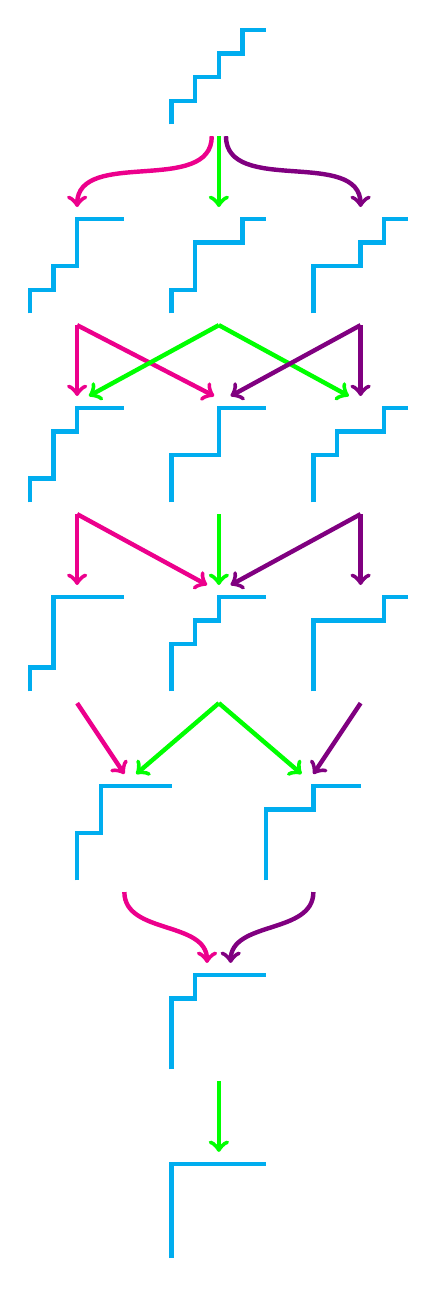
\begin{tikzpicture}[scale = 0.3]
    \draw [ultra thick, color = cyan] (0,0) -- (0,1)
        -- (0,2) -- (0,3) -- (0,4) -- (1,4) -- (2,4)
        -- (3,4) -- (4,4);

    \draw [ultra thick, color = cyan] (0,8) -- (0,9)
        -- (0,10) -- (0,11) -- (1,11) -- (1,12) -- (2,12)
        -- (3,12) -- (4,12);
        
    \draw [ultra thick, color = cyan] (-4,16) -- (-4,17)
        -- (-4,18) -- (-3,18) -- (-3,19) -- (-3,20)
        -- (-2,20) -- (-1,20) -- (0,20);

    \draw [ultra thick, color = cyan] (4,16) -- (4,17)
        -- (4,18) -- (4,19) -- (5,19) -- (6,19) -- (6,20)
        -- (7,20) -- (8,20);

    \draw [ultra thick, color = cyan] (-6,24) -- (-6,25)
        -- (-5,25) -- (-5,26) -- (-5,27) -- (-5,28)
        -- (-4,28) -- (-3,28) -- (-2,28);

    \draw [ultra thick, color = cyan] (0,24) -- (0,25)
        -- (0,26) -- (1,26) -- (1,27) -- (2,27) -- (2,28)
        -- (3,28) -- (4,28);

    \draw [ultra thick, color = cyan] (6,24) -- (6,25)
        -- (6,26) -- (6,27) -- (7,27) -- (8,27) -- (9,27)
        -- (9,28) -- (10,28);

    \draw [ultra thick, color = cyan] (-6,32) -- (-6,33)
        -- (-5,33) -- (-5,34) -- (-5,35) -- (-4,35)
        -- (-4,36) -- (-3,36) -- (-2,36);

    \draw [ultra thick, color = cyan] (0,32) -- (0,33)
        -- (0,34) -- (1,34) -- (2,34) -- (2,35) -- (2,36)
        -- (3,36) -- (4,36);

    \draw [ultra thick, color = cyan] (6,32) -- (6,33)
        -- (6,34) -- (7,34) -- (7,35) -- (8,35) -- (9,35)
        -- (9,36) -- (10,36);

    \draw [ultra thick, color = cyan] (-6,40) -- (-6,41)
        -- (-5,41) -- (-5,42) -- (-4,42) -- (-4,43)
        -- (-4,44) -- (-3,44) -- (-2,44);

    \draw [ultra thick, color = cyan] (0,40) -- (0,41)
        -- (1,41) -- (1,42) -- (1,43) -- (2,43) -- (3,43)
        -- (3,44) -- (4,44);

    \draw [ultra thick, color = cyan] (6,40) -- (6,41)
        -- (6,42) -- (7,42) -- (8,42) -- (8,43) -- (9,43)
        -- (9,44) -- (10,44);

    \draw [ultra thick, color = cyan] (0,48) -- (0,49)
        -- (1,49) -- (1,50) -- (2,50) -- (2,51) -- (3,51)
        -- (3,52) -- (4,52);


    \draw [->][out=-90,in=90, ultra thick] 
        [color=magenta](1.7,47.5) to (-4,44.5);
    \draw [->][color=magenta, ultra thick]
        (-4,39.5) to (-4,36.5);
    \draw [->][color=magenta, ultra thick]
        (-4,39.5) to (1.8,36.5); 
    \draw [->][color=magenta, ultra thick]
        (-4,31.5) to (-4,28.5);
    \draw [->][color=magenta, ultra thick]
        (-4,31.5) to (1.5,28.5);
    \draw [->][color=magenta, ultra thick]
        (-4,23.5) to (-2,20.5);
    \draw [->][out=-90,in=90, ultra thick] 
        [color=magenta](-2,15.5) to (1.5,12.5);


    \draw [->][out=-90,in=90, ultra thick]
        [color=green](2,47.5) to (2,44.5);
    \draw [->][color=green, ultra thick]
        (2,39.5) to (-3.5,36.5);
    \draw [->][color=green, ultra thick]
        (2,39.5) to (7.5,36.5);
    \draw [->][color=green, ultra thick]
        (2,31.5) to (2,28.5);
    \draw [->][color=green, ultra thick]
        (2,23.5) to (-1.5,20.5);
    \draw [->][color=green, ultra thick]
        (2,23.5) to (5.5,20.5);
    \draw [->][out=-90,in=90, ultra thick] 
        [color=green](2,7.5) to (2,4.5);

    \draw [->][out=-90,in=90, ultra thick]
        [color=violet](2.3,47.5) to (8,44.5);
    \draw [->][color=violet, ultra thick]
        (8,39.5) to (2.5,36.5);
    \draw [->][color=violet, ultra thick]
        (8,39.5) to (8,36.5);
    \draw [->][color=violet, ultra thick]
        (8,31.5) to (2.5,28.5);
    \draw [->][color=violet, ultra thick]
        (8,31.5) to (8,28.5);
    \draw [->][color=violet, ultra thick]
        (8,23.5) to (6,20.5);
    \draw [->][out=-90,in=90, ultra thick] 
        [color=violet](6,15.5) to (2.5,12.5);

\end{tikzpicture}
~\\
~\\
        There are $\frac {1}{5} \binom{8}{4} = \frac{70}{5} = 14$
        elements in this poset.
    \end{center}
\end{example}

\begin{definition}[Nested Dyck paths]
    Two Dyck Paths $w_1$ and $w_2$ are said \emph{nested}
    if $w_1$ is equal to $w_2$ or over $w_2$. 
\end{definition}

\begin{prop}
    If there exists a sequence $w_1 \gtrdot_d w_2 \gtrdot_d
    w_3 \gtrdot_d \cdots \gtrdot_d w_k$ with $k \geqslant 0$,
    then $w_1$ and $w_k$ are \emph{nested}.
\end{prop}

\begin{definition}[$\gtrdot'$]
    For $f$ and $g$ two primitive parking functions, we say
    that $f$ covers $g$, written $f \gtrdot' g$, if
    $\exists i$ such that :
    \begin{itemize}
        \item $f = (a_1, \ldots, a_{i-1}, a_i,\ \ \ \ 
            a_{i+1}, \ldots, a_n)$
        \item $g = (a_1, \ldots, a_{i-1}, a_i - 1, a_{i+1},
        \ldots, a_n)$
    \end{itemize}
\end{definition}

\begin{example}[$n = 6$]
    $(1, 1, 2, 3, 4, 5) \gtrdot' (1, 1, 2, 3, 3, 5)$    
\end{example}

\begin{prop}
    This covering relation defines a \emph{poset}
    for $\mathcal{PF'}_n$.
\end{prop}

\begin{example}[The poset of $\mathcal{PF'}_4$]
    ~\\
    \begin{center}
        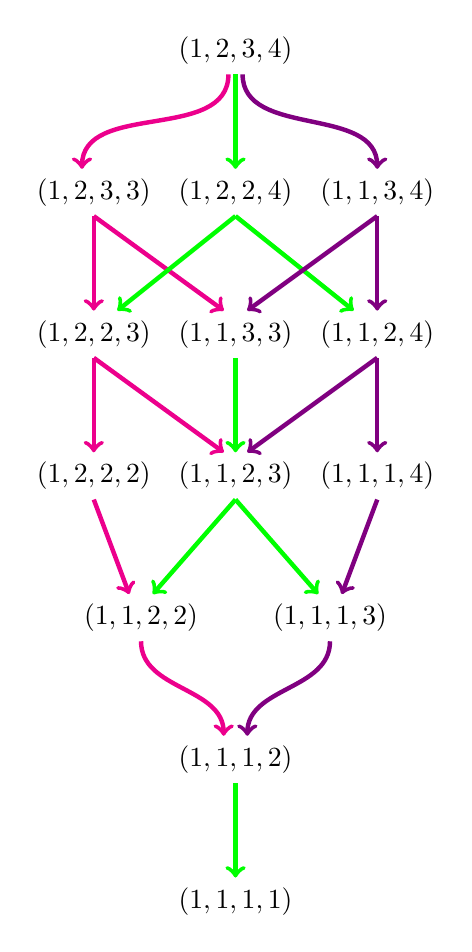
\begin{tikzpicture}[scale = 0.3]
    \node at (0,0)   {$(1,1,1,1)$};
    \node at (0,6)   {$(1,1,1,2)$};                
    \node at (-4,12) {$(1,1,2,2)$};
    \node at (4,12)  {$(1,1,1,3)$};
    \node at (-6,18) {$(1,2,2,2)$};
    \node at (0,18)  {$(1,1,2,3)$};
    \node at (6,18)  {$(1,1,1,4)$};
    \node at (-6,24) {$(1,2,2,3)$};
    \node at (0,24)  {$(1,1,3,3)$};
    \node at (6,24)  {$(1,1,2,4)$};
    \node at (-6,30) {$(1,2,3,3)$};
    \node at (0,30)  {$(1,2,2,4)$};
    \node at (6,30)  {$(1,1,3,4)$};
    \node at (0,36)  {$(1,2,3,4)$};


    \draw [->][out=-90,in=90, ultra thick] 
        [color=magenta](-0.3,35) to (-6.5,31);
    \draw [->][color=magenta, ultra thick]
        (-6,29) to (-6,25);
    \draw [->][color=magenta, ultra thick]
        (-6,29) to (-0.5,25); 
    \draw [->][color=magenta, ultra thick]
        (-6,23) to (-6,19);
    \draw [->][color=magenta, ultra thick]
        (-6,23) to (-0.5,19);
    \draw [->][color=magenta, ultra thick]
        (-6,17) to (-4.5,13);
    \draw [->][out=-90,in=90, ultra thick] 
        [color=magenta](-4,11) to (-0.5,7);


    \draw [->][out=-90,in=90, ultra thick]
        [color=green](0,35) to (0,31);
    \draw [->][color=green, ultra thick]
        (0,29) to (-5,25);
    \draw [->][color=green, ultra thick]
        (0,29) to (5,25);
    \draw [->][color=green, ultra thick]
        (0,23) to (0,19);
    \draw [->][color=green, ultra thick]
        (0,17) to (-3.5,13);
    \draw [->][color=green, ultra thick]
        (0,17) to (3.5,13);
    \draw [->][out=-90,in=90, ultra thick] 
        [color=green](0,5) to (0,1);

    \draw [->][out=-90,in=90, ultra thick]
        [color=violet](0.3,35) to (6,31);
    \draw [->][color=violet, ultra thick]
        (6,29) to (0.5,25);
    \draw [->][color=violet, ultra thick]
        (6,29) to (6,25);
    \draw [->][color=violet, ultra thick]
        (6,23) to (0.5,19);
    \draw [->][color=violet, ultra thick]
        (6,23) to (6,19);
    \draw [->][color=violet, ultra thick]
        (6,17) to (4.5,13);
    \draw [->][out=-90,in=90, ultra thick] 
        [color=violet](4,11) to (0.5,7);

\end{tikzpicture}
~\\
~\\
        There are $\frac {1}{5} \binom{8}{4} = \frac{70}{5} = 14$
        elements in this poset.
    \end{center}
\end{example}

\begin{rem}
    The two posets are isomorphic, and one can be obtained by
    applying the aforementioned bijection to the other.
\end{rem}

\begin{theorem}
    The number of intervals in those posets is equal to
    the $n+1^{th}$ term of the integer sequence defined by
    https://oeis.org/A005700.\\
    The first terms of this sequence are $1, 1, 3, 14, 84,
    594, 4719, 40898, 379236, 3711916, ...$\\
    Alec Mihailovs proved this sequence to be equal to
    $$\frac {6 (2n)! (2n+2)!}{n!(n+1)!(n+2)!(n+3)!}$$.
\end{theorem}

\begin{proof}
    As the number of intervals in the poset for Dyck words
    can be seen as the number of pairs $(w_1, w_k)$ such that
    $w_1 \gtrdot_d w_2 \gtrdot_d \cdots \gtrdot_d w_k$, we can
    define it as the number of \emph{nested pairs of Dyck paths}.
    This has been proved to be equal to this integer sequence by
    Bruce Westbury in 2013.
\end{proof}

\subsubsection{Classical Dyck - Parking Posets}

\begin{definition}[$\gtrdot_{ld}$]
    For $w$ and $w'$ two labeled Dyck words, we say
    that $w$ covers $w'$, written $w \gtrdot_{ld} w'$,
    if $\exists l, r, x, x', y, z, z'$ such that :
    \begin{itemize}
        \item $l$ is either empty or ends with $0$
        \item $r$ is either empty or starts with $0$
        \item $x = x_1x_2 \cdots$ has all its digits $> 0$
        \item $z = z_1z_2 \cdots$ has all its digits $> 0$
        \item $x' = x$ where $y$ is correctly inserted
            regarding the order condition
        \item $y$ is in $z$, and $z' = z$ where $y$ is removed
        \item $w = lx0zr$
        \item $w' = lx'0z'r$
    \end{itemize}  
\end{definition}

\begin{example}[$n = 5$]
    $104503600200 \gtrdot_{ld} 10345060200$
    \begin{itemize}
        \item $l = 10$
        \item $r = 0200$
        \item $x = 45$
        \item $x' = 345$
        \item $y = 3$
        \item $z = 36$
        \item $z' = 6$
    \end{itemize}
    \begin{center}
    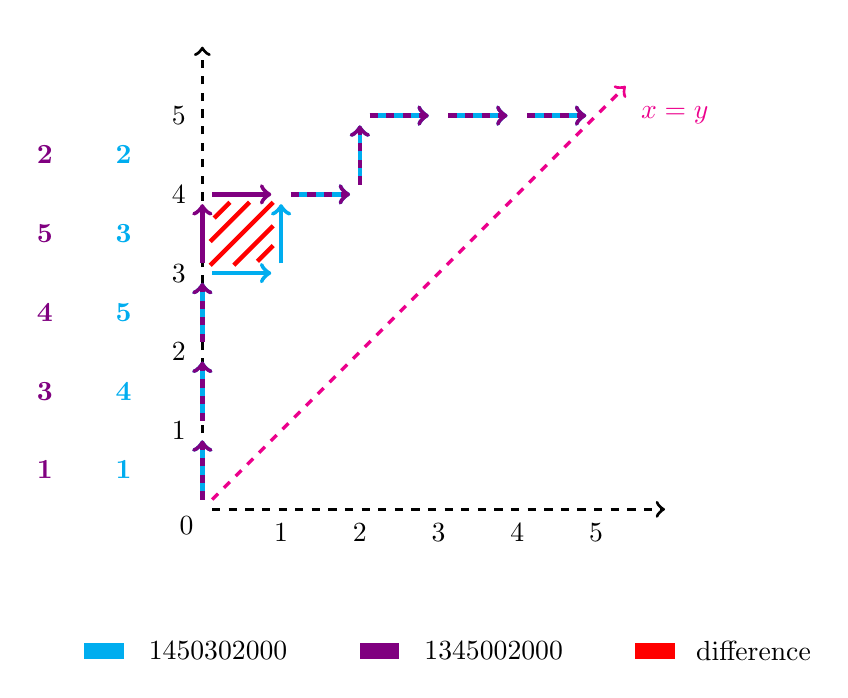
\begin{tikzpicture}[scale=1]
        \node (a) at (0, 0) {};
        \node (b) at (0, 6) {};
        \node (c) at (6, 0) {};
        \node (d) at (5.5, 5.5) {};
        \node (e) at (6, 5) [color = magenta]
            {$x = y$}; 
        \draw [dashed, very thick, ->] (a) to (b);
        \draw [dashed, very thick, ->] (a) to (c);
        \draw [dashed, very thick, ->]
            [color = magenta] (a) to (d);

        \node (1)  at (0,0)   {};
        \node (2)  at (0,1)   {};
        \node (3)  at (0,2)   {};
        \node (4)  at (0,3)   {};
        \node (5)  at (1,3)   {};
        \node (5b) at (0,4)   {};
        \node (6)  at (1,4)   {};
        \node (7)  at (2,4)   {};
        \node (8)  at (2,5)   {};
        \node (9)  at (3,5)   {};
        \node (10) at (4,5)   {};
        \node (11) at (5,5)   {};

        \draw [->, ultra thick, color = cyan]
            (1)  to (2);
        \draw [->, ultra thick, color = cyan] 
            (2)  to (3);
        \draw [->, ultra thick, color = cyan]
            (3)  to (4);
        \draw [->, ultra thick, color = cyan]
            (4)  to (5);
        \draw [->, ultra thick, color = cyan]
            (5)  to (6);
        \draw [->, ultra thick, color = cyan]
            (6)  to (7);
        \draw [->, ultra thick, color = cyan]
            (7)  to (8);
        \draw [->, ultra thick, color = cyan]
            (8)  to (9);
        \draw [->, ultra thick, color = cyan]
            (9)  to (10);
        \draw [->, ultra thick, color = cyan]
            (10) to (11);

        \draw [->, dashed, ultra thick, color = violet]
            (1)  to (2);
        \draw [->, dashed, ultra thick, color = violet] 
            (2)  to (3);
        \draw [->, dashed, ultra thick, color = violet]
            (3)  to (4);
        \draw [->, ultra thick, color = violet]
            (4)  to (5b);
        \draw [->, ultra thick, color = violet]
            (5b)  to (6);
        \draw [->, dashed, ultra thick, color = violet]
            (6)  to (7);
        \draw [->, dashed, ultra thick, color = violet]
            (7)  to (8);
        \draw [->, dashed, ultra thick, color = violet]
            (8)  to (9);
        \draw [->, dashed, ultra thick, color = violet]
            (9)  to (10);
        \draw [->, dashed, ultra thick, color = violet]
            (10) to (11);

        \node at (-0.2, -0.2) {$0$};
        \node at (-0.3, 1)    {$1$};
        \node at (1, -0.3)    {$1$};
        \node at (-0.3, 2)    {$2$};
        \node at (2, -0.3)    {$2$};
        \node at (-0.3, 3)    {$3$};
        \node at (3, -0.3)    {$3$};
        \node at (-0.3, 4)    {$4$};
        \node at (4, -0.3)    {$4$};
        \node at (-0.3, 5)    {$5$};
        \node at (5, -0.3)    {$5$};


        \node [color = cyan] at (-1, 0.5) {\textbf{1}};
        \node [color = cyan] at (-1, 1.5) {\textbf{4}};
        \node [color = cyan] at (-1, 2.5) {\textbf{5}};
        \node [color = cyan] at (-1, 3.5) {\textbf{3}};
        \node [color = cyan] at (-1, 4.5) {\textbf{2}};


        \node [color = violet] at (-2, 0.5) {\textbf{1}};
        \node [color = violet] at (-2, 1.5) {\textbf{3}};
        \node [color = violet] at (-2, 2.5) {\textbf{4}};
        \node [color = violet] at (-2, 3.5) {\textbf{5}};
        \node [color = violet] at (-2, 4.5) {\textbf{2}};

        \draw[color = red, ultra thick]
            (0.1,3.1) -- (0.9,3.9);
        \draw[color = red, ultra thick]
            (0.1,3.4) -- (0.6,3.9);
        \draw[color = red, ultra thick]
            (0.15,3.7) -- (0.35,3.9);
        \draw[color = red, ultra thick]
            (0.4,3.1) -- (0.9,3.6);
        \draw[color = red, ultra thick]
            (0.7,3.15) -- (0.9,3.35);

        \fill[color = cyan] (-1,-1.9) rectangle
            (-1.5,-1.7);
        \node at (0.2,-1.8) {$1450302000$};
        \fill[color = violet] (2,-1.9) rectangle
            (2.5,-1.7);
        \node at (3.7,-1.8) {$1345002000$};
        \fill[color = red] (6,-1.9) rectangle
            (5.5,-1.7);
        \node at (7,-1.8) {difference};
    \end{tikzpicture}
\end{center}
\end{example}

\begin{definition}[Rise]
    A \emph{rise} of a decorated Dyck word is a maximal
    sequence of non-zero digits preceding a zero.
\end{definition}

\begin{example}[$n = 5$]
    In order, the rises of $104503600200$ are :\\
    \begin{itemize*}
        \item $1$
        \item $45$
        \item $36$
        \item $\emptyset$
        \item $2$
        \item $\emptyset$
    \end{itemize*}
\end{example}

\begin{rem}
    If $w_1 \gtrdot_{ld} w_2$, then the path corresponding to
    $w_2$ is \emph{over} the path corresponding to $w_1$,
    and the \emph{difference} between the two paths is a
    square of size 1 by 1.\\
    Furthermore, the covering relation can be seen as follows :
    $w_1$ covers $w_2$ if we can obtain $w_2$ by taking a
    digit from the $i + 1^{th}$ rise of $w_1$, and inserting it
    into the $i^{th}$ rise of $w_1$ in increasing order.
\end{rem}

\begin{prop}
    This covering relation defines a \emph{poset}
    for $\mathcal{LD}_n$.
\end{prop}

\begin{example}[The poset of $\mathcal{LD}_3$]
    ~\\
    \begin{center}
        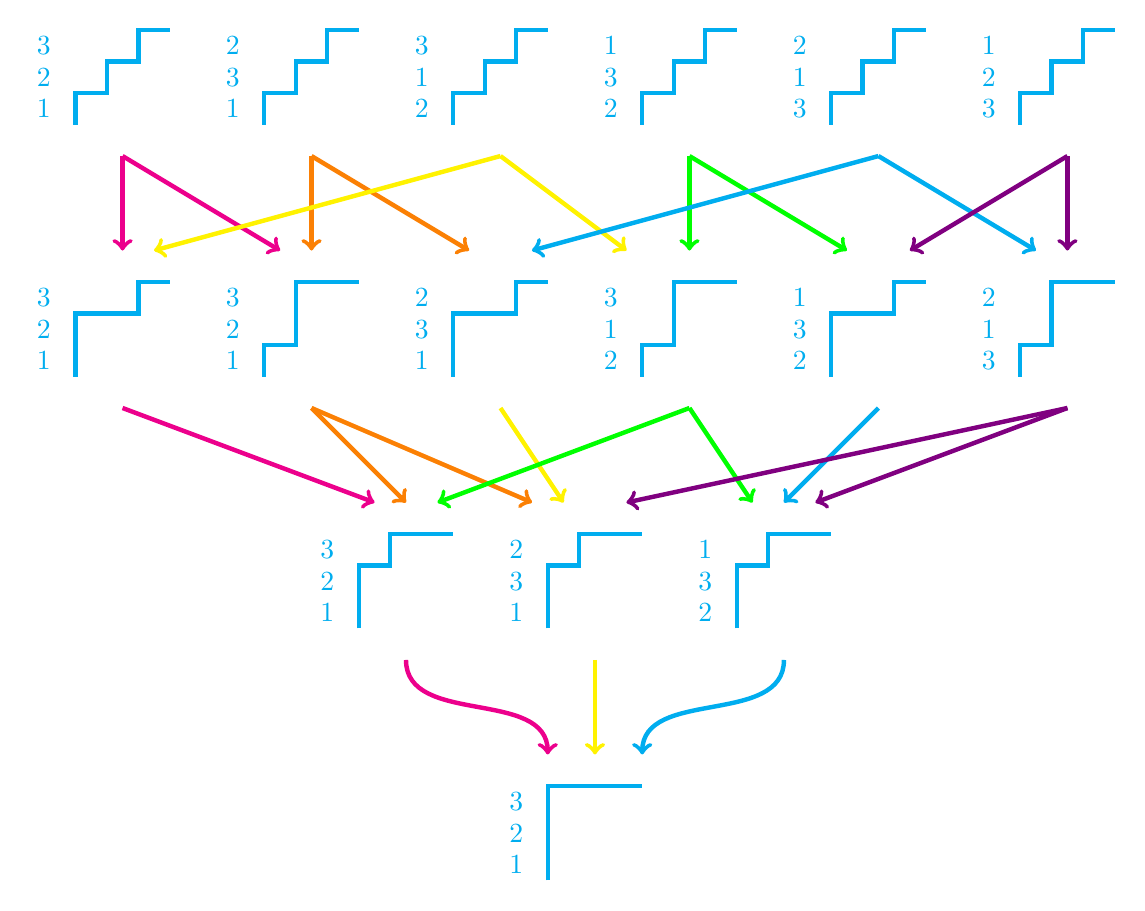
\begin{tikzpicture}[scale = 0.4]
    \draw [ultra thick, color = cyan] (0,0) -- (0,1)
        -- (0,2) -- (0,3) -- (1,3) -- (2,3) -- (3,3);
    \node[color = cyan] at (-1,0.5) {$1$};
    \node[color = cyan] at (-1,1.5) {$2$};
    \node[color = cyan] at (-1,2.5) {$3$};

    \draw [ultra thick, color = cyan] (-6,8) -- (-6,9)
        -- (-6,10) -- (-5,10) -- (-5,11) -- (-4,11)
        -- (-3,11);
    \node[color = cyan] at (-7,8.5) {$1$};
    \node[color = cyan] at (-7,9.5) {$2$};
    \node[color = cyan] at (-7,10.5) {$3$};
        
    \draw [ultra thick, color = cyan] (0,8) -- (0,9)
        -- (0,10) -- (1,10) -- (1,11) -- (2,11)
        -- (3,11);
    \node[color = cyan] at (-1,8.5) {$1$};
    \node[color = cyan] at (-1,9.5) {$3$};
    \node[color = cyan] at (-1,10.5) {$2$};

    \draw [ultra thick, color = cyan] (6,8) -- (6,9)
        -- (6,10) -- (7,10) -- (7,11) -- (8,11)
         -- (9,11);
    \node[color = cyan] at (5,8.5) {$2$};
    \node[color = cyan] at (5,9.5) {$3$};
    \node[color = cyan] at (5,10.5) {$1$};

    \draw [ultra thick, color = cyan] (-15,16) -- (-15,17)
        -- (-15,18) -- (-14,18) -- (-13,18) -- (-13,19)
        -- (-12,19);
    \node[color = cyan] at (-16,16.5) {$1$};
    \node[color = cyan] at (-16,17.5) {$2$};
    \node[color = cyan] at (-16,18.5) {$3$};

    \draw [ultra thick, color = cyan] (-9,16) -- (-9,17)
        -- (-8,17) -- (-8,18) -- (-8,19) -- (-7,19)
        -- (-6,19);
    \node[color = cyan] at (-10,16.5) {$1$};
    \node[color = cyan] at (-10,17.5) {$2$};
    \node[color = cyan] at (-10,18.5) {$3$};

    \draw [ultra thick, color = cyan] (-3,16) -- (-3,17)
        -- (-3,18) -- (-2,18) -- (-1,18) -- (-1,19)
        -- (0,19);
    \node[color = cyan] at (-4,16.5) {$1$};
    \node[color = cyan] at (-4,17.5) {$3$};
    \node[color = cyan] at (-4,18.5) {$2$};

    \draw [ultra thick, color = cyan] (3,16) -- (3,17)
        -- (4,17) -- (4,18) -- (4,19) -- (5,19)
        -- (6,19);
    \node[color = cyan] at (2,16.5) {$2$};
    \node[color = cyan] at (2,17.5) {$1$};
    \node[color = cyan] at (2,18.5) {$3$};

    \draw [ultra thick, color = cyan] (9,16) -- (9,17)
        -- (9,18) -- (10,18) -- (11,18) -- (11,19)
        -- (12,19);
    \node[color = cyan] at (8,16.5) {$2$};
    \node[color = cyan] at (8,17.5) {$3$};
    \node[color = cyan] at (8,18.5) {$1$};

    \draw [ultra thick, color = cyan] (15,16) -- (15,17)
        -- (16,17) -- (16,18) -- (16,19) -- (17,19)
        -- (18,19);
    \node[color = cyan] at (14,16.5) {$3$};
    \node[color = cyan] at (14,17.5) {$1$};
    \node[color = cyan] at (14,18.5) {$2$};

    \draw [ultra thick, color = cyan] (-15,24) -- (-15,25)
        -- (-14,25) -- (-14,26) -- (-13,26) -- (-13,27)
        -- (-12,27);
    \node[color = cyan] at (-16,24.5) {$1$};
    \node[color = cyan] at (-16,25.5) {$2$};
    \node[color = cyan] at (-16,26.5) {$3$};

    \draw [ultra thick, color = cyan] (-9,24) -- (-9,25)
        -- (-8,25) -- (-8,26) -- (-7,26) -- (-7,27)
        -- (-6,27);
    \node[color = cyan] at (-10,24.5) {$1$};
    \node[color = cyan] at (-10,25.5) {$3$};
    \node[color = cyan] at (-10,26.5) {$2$};

    \draw [ultra thick, color = cyan] (-3,24) -- (-3,25)
        -- (-2,25) -- (-2,26) -- (-1,26) -- (-1,27)
        -- (0,27);
    \node[color = cyan] at (-4,24.5) {$2$};
    \node[color = cyan] at (-4,25.5) {$1$};
    \node[color = cyan] at (-4,26.5) {$3$};


    \draw [ultra thick, color = cyan] (3,24) -- (3,25)
        -- (4,25) -- (4,26) -- (5,26) -- (5,27)
        -- (6,27);
    \node[color = cyan] at (2,24.5) {$2$};
    \node[color = cyan] at (2,25.5) {$3$};
    \node[color = cyan] at (2,26.5) {$1$};

    \draw [ultra thick, color = cyan] (9,24) -- (9,25)
        -- (10,25) -- (10,26) -- (11,26) -- (11,27)
        -- (12,27);
    \node[color = cyan] at (8,24.5) {$3$};
    \node[color = cyan] at (8,25.5) {$1$};
    \node[color = cyan] at (8,26.5) {$2$};

    \draw [ultra thick, color = cyan] (15,24) -- (15,25)
        -- (16,25) -- (16,26) -- (17,26) -- (17,27)
        -- (18,27);
    \node[color = cyan] at (14,24.5) {$3$};
    \node[color = cyan] at (14,25.5) {$2$};
    \node[color = cyan] at (14,26.5) {$1$};

    \draw [->][color=magenta, ultra thick]
        (-13.5,23) to (-13.5,20);
    \draw [->][color=magenta, ultra thick]
        (-13.5,23) to (-8.5,20);
    \draw [->][color=magenta, ultra thick]
        (-13.5,15) to (-5.5,12); 
    \draw [->][out=-90,in=90, ultra thick] 
        [color=magenta](-4.5,7) to (0,4);

    \draw [->][color=brown!7!orange, ultra thick]
        (-7.5,23) to (-7.5,20);
    \draw [->][color=brown!7!orange, ultra thick]
        (-7.5,23) to (-2.5,20);
    \draw [->][color=brown!7!orange, ultra thick]
        (-7.5,15) to (-4.5,12);
    \draw [->][color=brown!7!orange, ultra thick]
        (-7.5,15) to (-0.5,12);

    \draw [->][color=yellow, ultra thick]
        (-1.5,23) to (-12.5,20);
    \draw [->][color=yellow, ultra thick]
        (-1.5,23) to (2.5,20);
    \draw [->][color=yellow, ultra thick]
        (-1.5,15) to (0.5,12); 
    \draw [->][out=-90,in=90, ultra thick] 
        [color=yellow](1.5,7) to (1.5,4);

    \draw [->][color = green,  ultra thick]
        (4.5,23) to (4.5,20);
    \draw [->][color=green, ultra thick]
        (4.5,23) to (9.5,20);
    \draw [->][color=green, ultra thick]
        (4.5,15) to (-3.5,12);
    \draw [->][color=green, ultra thick]
        (4.5,15) to (6.5,12);

    \draw [->][color=cyan, ultra thick]
        (10.5,23) to (-0.5,20);
    \draw [->][color=cyan, ultra thick]
        (10.5,23) to (15.5,20);
    \draw [->][color=cyan, ultra thick]
        (10.5,15) to (7.5,12); 
    \draw [->][out=-90,in=90, ultra thick] 
        [color=cyan](7.5,7) to (3,4);

    \draw [->][color=violet, ultra thick]
        (16.5,23) to (11.5,20);
    \draw [->][color=violet, ultra thick]
        (16.5,23) to (16.5,20);
    \draw [->][color=violet, ultra thick]
        (16.5,15) to (2.5,12);
    \draw [->][color=violet, ultra thick]
        (16.5,15) to (8.5,12);

\end{tikzpicture}
~\\
~\\
        There are $4^2 = 16$ elements in this poset.
    \end{center}
\end{example}

\begin{definition}[$\gtrdot$]
    For $f$ and $g$ two parking functions, we say
    that $f$ covers $g$, written $f \gtrdot g$, if
    $\exists i$ such that :
    \begin{itemize}
        \item $f = (a_1, \ldots, a_{i-1}, a_i,\ \ \ \ 
            a_{i+1}, \ldots, a_n)$
        \item $g = (a_1, \ldots, a_{i-1}, a_i - 1, a_{i+1},
        \ldots, a_n)$
    \end{itemize}
    That is, the same relation as for primitive
    parking functions.
\end{definition}

\begin{example}[$n = 6$]
    $(2, 1, 5, 3, 1, 4) \gtrdot (2, 1, 5, 2, 1, 4)$    
\end{example}

\begin{prop}
    This covering relation defines a \emph{poset}
    for $\mathcal{PF}_n$.
\end{prop}

\begin{example}[The poset of $\mathcal{PF}_3$]
    ~\\
    \begin{center}
        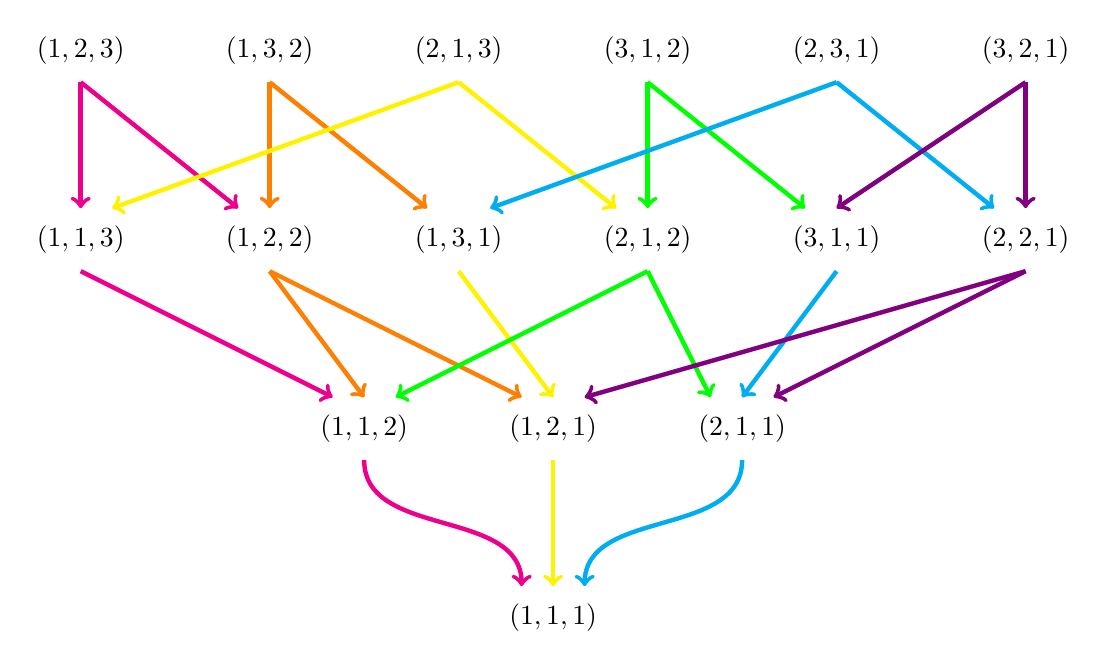
\begin{tikzpicture}[scale = 0.4]
    \node at (0,0) {$(1,1,1)$};

    \node at (-6,6) {$(1,1,2)$};                
    \node at (0,6)  {$(1,2,1)$};
    \node at (6,6)  {$(2,1,1)$};

    \node at (-15,12) {$(1,1,3)$};
    \node at (-9,12)  {$(1,2,2)$};
    \node at (-3,12)  {$(1,3,1)$};
    \node at (3,12)   {$(2,1,2)$};
    \node at (9,12)   {$(3,1,1)$};
    \node at (15,12)  {$(2,2,1)$};

    \node at (-15,18) {$(1,2,3)$};
    \node at (-9,18)  {$(1,3,2)$};
    \node at (-3,18)  {$(2,1,3)$};
    \node at (3,18)   {$(3,1,2)$};
    \node at (9,18)   {$(2,3,1)$};
    \node at (15,18)  {$(3,2,1)$};

    \draw [->][color=magenta, ultra thick]
        (-15,17) to (-15,13);
    \draw [->][color=magenta, ultra thick]
        (-15,17) to (-10,13);
    \draw [->][color=magenta, ultra thick]
        (-15,11) to (-7,7); 
    \draw [->][out=-90,in=90, ultra thick] 
        [color=magenta](-6,5) to (-1,1);

    \draw [->][color=brown!7!orange, ultra thick]
        (-9,17) to (-9,13);
    \draw [->][color=brown!7!orange, ultra thick]
        (-9,17) to (-4,13);
    \draw [->][color=brown!7!orange, ultra thick]
        (-9,11) to (-6,7);
    \draw [->][color=brown!7!orange, ultra thick]
        (-9,11) to (-1,7);

    \draw [->][color=yellow, ultra thick]
        (-3,17) to (-14,13);
    \draw [->][color=yellow, ultra thick]
        (-3,17) to (2,13);
    \draw [->][color=yellow, ultra thick]
        (-3,11) to (0,7); 
    \draw [->][out=-90,in=90, ultra thick] 
        [color=yellow](0,5) to (0,1);

    \draw [->][color = green,  ultra thick]
        (3,17) to (3,13);
    \draw [->][color=green, ultra thick]
        (3,17) to (8,13);
    \draw [->][color=green, ultra thick]
        (3,11) to (-5,7);
    \draw [->][color=green, ultra thick]
        (3,11) to (5,7);

    \draw [->][color=cyan, ultra thick]
        (9,17) to (-2,13);
    \draw [->][color=cyan, ultra thick]
        (9,17) to (14,13);
    \draw [->][color=cyan, ultra thick]
        (9,11) to (6,7); 
    \draw [->][out=-90,in=90, ultra thick] 
        [color=cyan](6,5) to (1,1);

    \draw [->][color=violet, ultra thick]
        (15,17) to (9,13);
    \draw [->][color=violet, ultra thick]
        (15,17) to (15,13);
    \draw [->][color=violet, ultra thick]
        (15,11) to (1,7);
    \draw [->][color=violet, ultra thick]
        (15,11) to (7,7);

\end{tikzpicture}
~\\
~\\
        There are $4^2 = 16$ elements in this poset.
    \end{center}
\end{example}

\begin{rem}
    The two posets are isomorphic, and one can be obtained by
    applying the aforementioned bijection to the other.
\end{rem}

\begin{conj}
    The number of intervals in those posets is equal to
    the $n+1^{th}$ term of the integer sequence defined by
    https://oeis.org/A196304.\\
    The first terms of this sequence are $1, 1, 5, 64, 1587,
    65421, 4071178, 357962760, 4237910716, ...$.
\end{conj}